%\section{Evaluation}
%\label{sec:experiments}
\subsection{Performance Metrics}
We evaluate PSWare based on the applications we have discussed before. In this sub-section, we introduce the performance metrics used in our evaluation.

The primary of PSWare is help developing WSN-based applications. However, additional overhead may be introduced by its event detection framework. Therefore, we use the following metrics to evaluate PSWare:
\begin{itemize}
\item Memory usage: since the sensor nodes have limited amount of memory, it is important to know the memory overhead introduced by PSWare in order to evaluate its practical use. 
\item Message cost: it is useful to measure the application message cost when using customized event processing mechanism. This way, we can show how PSWare is helpful in deploying real applications. The message cost is obtained by setting up a counter inside the sensor node. The counter will be written into flash so that we can retrieve it after the experiments.
\item Event detection delay: some event processing mechanisms aims at shortening the event detection delay. In this paper, we measure the time between the subscription is disseminated and the event is notified.
\end{itemize}

For each of the application case discussed in the previous section, we implemented an additional opportunistic event detection mechanism where all the events are transmitted to the sink for detection. The transmission is done using the existing routing protocol, CTP, provided by TinyOS. This serves as reference when studying the performance.

\subsection{Evaluation Results}
In the car park application, the messages indicating the occupancy of the cars must be reliably delivered to the control center. Therefore, we implemented a retransmission mechanism for event delivery. With PSware, the application takes 61k bytes of code and 1.5k bytes of data. Without PSWare, the application takes around 35k bytes for code and 1.3k bytes for data. For the evaluation, we primarily consider only the message costs because the delay isn't that important in such a system. The experimental results for the car park are shown in Figure \ref{fig:carParkResults}. The message cost is highest during rush hour when there are a lot of cars entering and leaving the car park. To further study application under different settings, we used two deployment strategies. The first one is even deployment, where all the parking spaces in a particular area are deployed. In the second strategy, we assume the management is only interested in a subset of the parking spaces so we randomly deployed the sensor nodes in some of the parking spaces. For all the experiments as we can see, the message cost by using application-specific middleware for ITS is the lowest while the opportunistic way is the highest.

\begin{figure}
\centering
\subfloat[With random fusion point deployment]{\label{fig:carParkResult1}\figurehalfwidth{carParkResult1}}
%\qquad
\subfloat[With even fusion point deployment]{\label{fig:carParkResult2}\figurehalfwidth{carParkResult2}}
\caption{Car park experiment results}
\label{fig:carParkResults}
\end{figure}

The next application we evaluate is ITS. One distinct feature of ITS is that we can make use of the special road deployment of the sensor nodes to make event processing easier. As a result, by replacing the default event processing algorithm with a simpler one that processes the event along the road, both code and data sizes are reduced. Without PSWare, the application takes around 25k bytes for code and 1.2k bytes for data. With PSware, it takes around 51k bytes of code and 1.4k bytes of data. The results for ITS are shown in Figure \ref{fig:itsResults}. Different from the car park application, such applications are more delay sensitive. So we also measured the time delay for the event detection. %Similar to the car park application, ITS-specific event detection mechanism can save most energy. Both ITS and TED will introduce certain amount of delay due to the waiting.
 
\begin{figure}
\centering
\subfloat[Message cost]{\label{fig:itsResult1}\figurehalfwidth{itsResult1}}
%\qquad
\subfloat[Delay]{\label{fig:itsResult2}\figurehalfwidth{itsResult2}}
\caption{Experiments on the roads}
\label{fig:itsResults}
\end{figure}

Our final experiments is for the indoor monitoring application. We consider the application scenario where the sensor nodes are deployed in a building so that the temperature can be monitored. With PSware, the application takes 58k bytes of code and 1.5k bytes of data. Without PSWare, the application takes around 34k bytes for code and 1.3k bytes for data. The application As discussed in the previous sections, such an application can probably be useful for certain types of context aware pervasive applications such as indoor temperature monitoring. The experimental results is shown in Figure \ref{fig:itsResults}. 

\begin{figure}
\centering
\subfloat[With random fusion point deployment]{\label{fig:indoorResult1}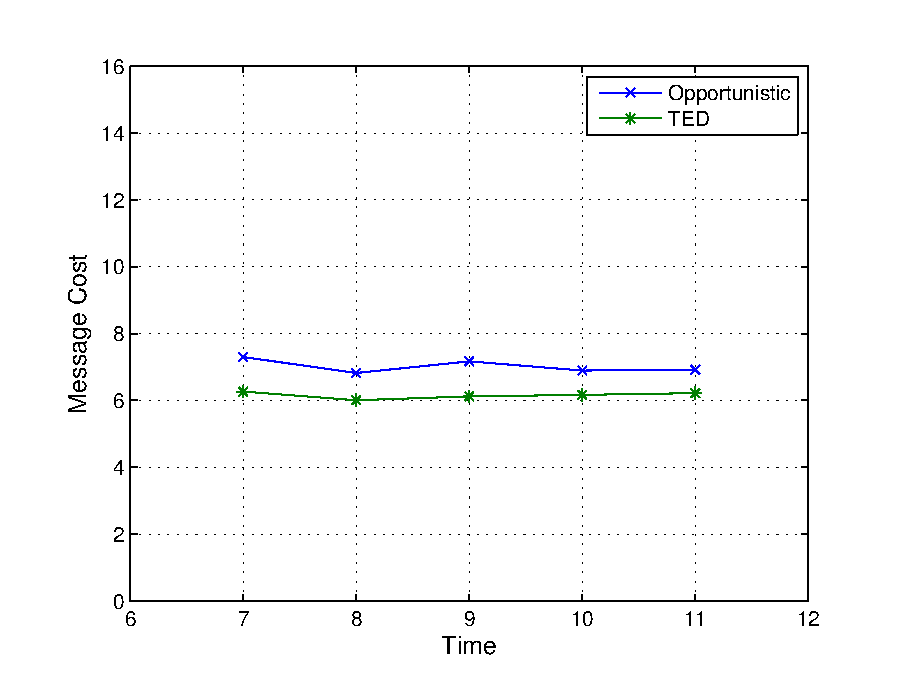
\includegraphics[width=.5\textwidth]{indoorResult1}}
%\qquad
\subfloat[With even fusion point deployment]{\label{fig:indoorResult2}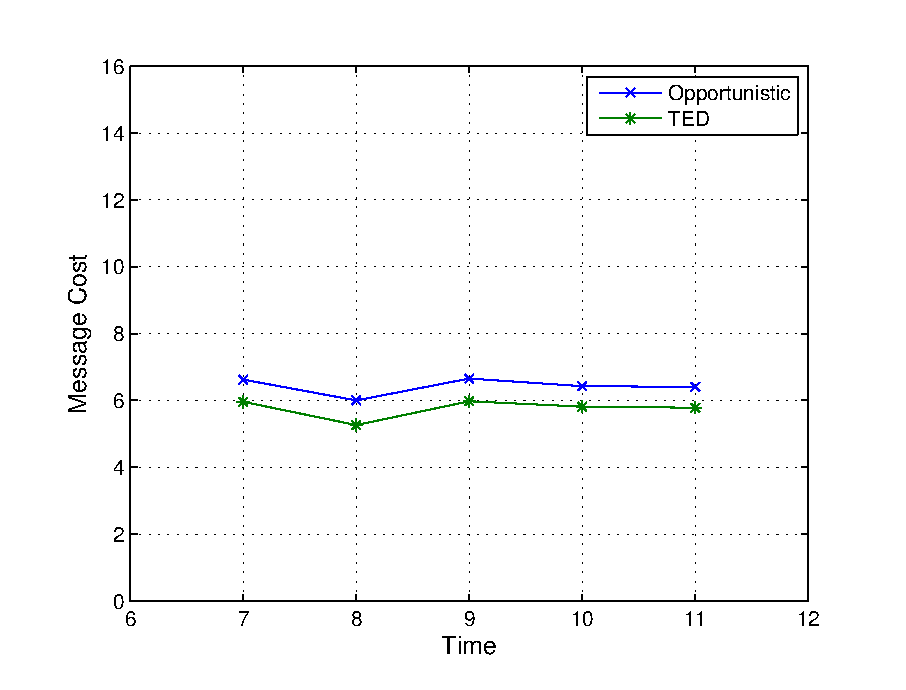
\includegraphics[width=.5\textwidth]{indoorResult2}}
\caption{Experiments for temperature monitoring}
\label{fig:indoorResult}
\end{figure}
